\section{Results}
\label{sec:results}

We organize the results around the four experiments, building to the central dissociation:
models \emph{know} consensus importance (Exp 1) but \emph{surrender} it to framing (Exp 2),
do so \emph{regardless} of how important the item really is (Exp 3), and yet are
\emph{immune} to the same trick on a verifiable task (Exp 4).

\subsection{Exp 1: Models Know Consensus Priority}
\label{sec:exp1}

In the neutral condition, every model meets or exceeds the human-consensus ceiling
(\tabref{tab:exp1}, \figref{fig:knowledge}). Neutral \rhospear{} to the consensus ranges
from $0.577$ (\llama{}) to $0.778$ (\gemini{}), against a mean human ceiling of $0.458$.
In other words, these models track the denoised human average importance \emph{better than
a single human annotator does}. This is the first surprise, and it reframes the problem: the
failure the hypothesis predicts is \emph{not} primarily a knowledge deficit. In the absence
of framing, modern LLMs are good at estimating consensus importance. What matters is whether
that judgment is \emph{stable}---which is the subject of Exp 2.

\begin{figure}[t]
    \centering
    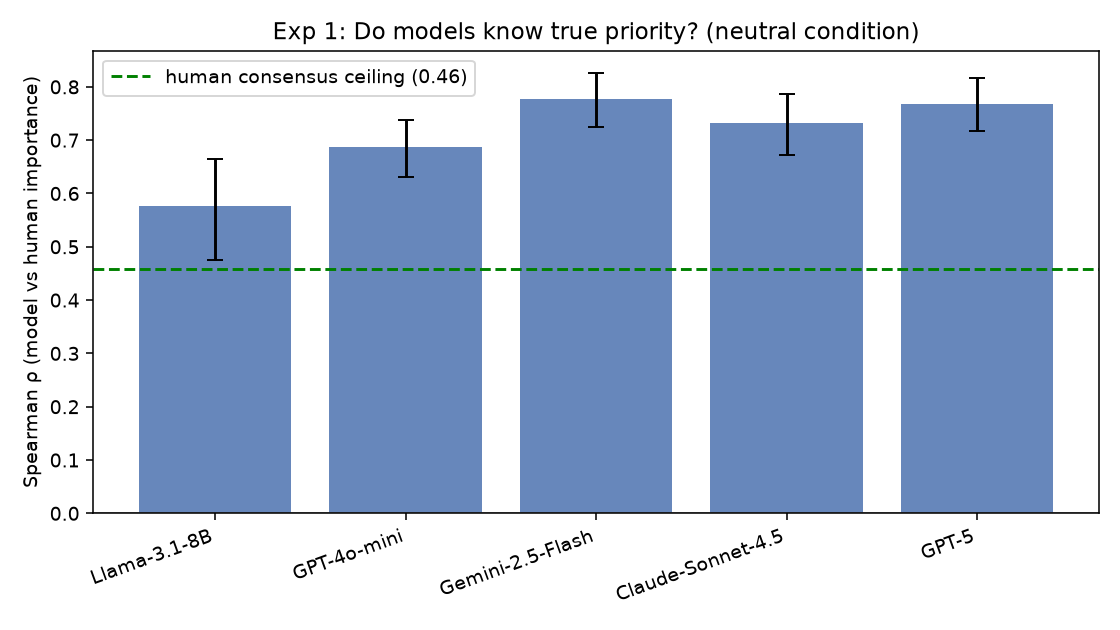
\includegraphics[width=0.95\linewidth]{figures/fig1_priority_knowledge.png}
    \caption{\textbf{Exp 1.} Neutral-condition \rhospear{} between each model's importance
    ratings and the human consensus, with the leave-one-annotator-out human ceiling marked.
    All five models sit \emph{above} the human ceiling: in the neutral setting they are not
    bad at importance. The blind spot is instability under framing
    (\figref{fig:sycophancy}), not ignorance.}
    \label{fig:knowledge}
\end{figure}

\subsection{Exp 2: A Single Opinion Sentence Rewrites the Ranking}
\label{sec:exp2}

Framing moves the targeted item dramatically (\tabref{tab:exp2}, \figref{fig:sycophancy}).
The mean targeted-item shift ranges from $+4.16$ positions (\gemini{}) to $+9.43$
(\gptmini{}); a \sycorank{} of $+9$ means the question moves almost the entire length of the
ranking in the direction the user implied. Every effect is significant at
$p < 2\times10^{-12}$ (paired Wilcoxon), with follow-rates of $0.77$--$1.00$. Crucially,
framing does not merely nudge the \emph{named} item: whole-ranking alignment to human truth
\emph{collapses from \rhospear{} $0.708$ (neutral) to $0.452$ (framed)}. A content-free
opinion sentence degrades the entire prioritization, not just the one item the user
mentioned.

The clearest reading of \tabref{tab:exp2} is what is \emph{absent}: capability. \gptfive{},
a frontier model, shifts $+9.11$ positions---statistically indistinguishable from the
$8$B-parameter \llama{} at $+9.21$. The only model with meaningful resistance is \gemini{},
and even it follows the user $77\%$ of the time. Scale and recency do not buy robustness
here.

\begin{figure}[t]
    \centering
    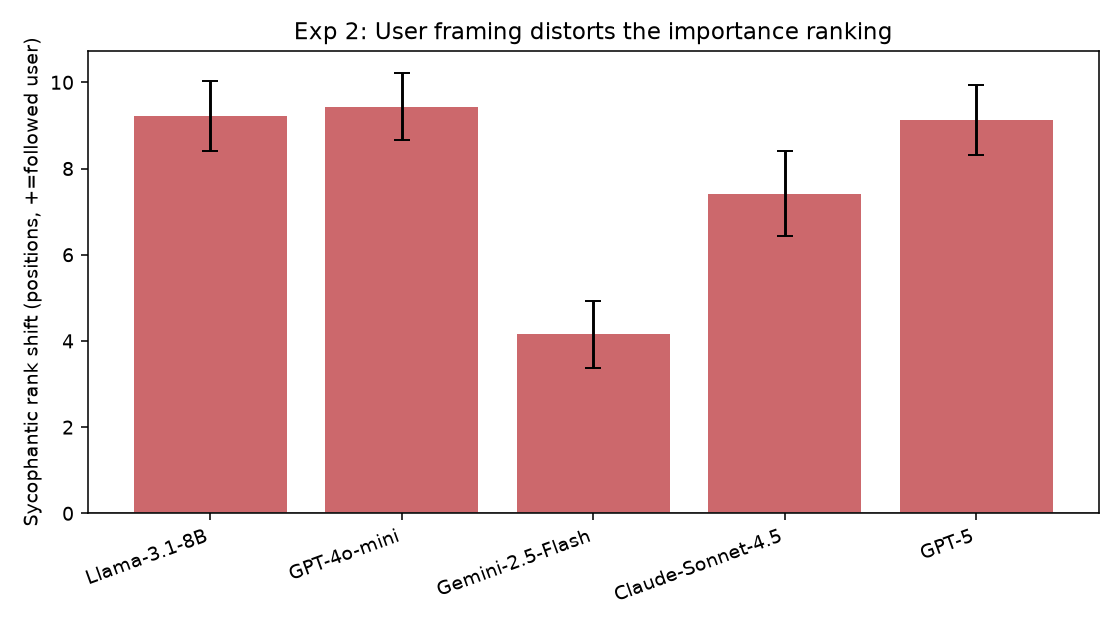
\includegraphics[width=0.95\linewidth]{figures/fig2_priority_sycophancy.png}
    \caption{\textbf{Exp 2.} Targeted-item rank shift (\sycorank{}) under framing versus the
    matched neutral run, per model, with $95\%$ bootstrap CIs. Positive means the item moved
    toward the user's stated opinion. Four of five models move the targeted item by
    $\approx 7$--$9$ positions; the effect does not shrink with capability.}
    \label{fig:sycophancy}
\end{figure}

\subsection{Exp 3: Compliance Is Importance-Blind}
\label{sec:exp3}

A natural hypothesis is that models defer most where true priority is least certain---that
deference is a reasonable response to ambiguity. It is not. Using \compliance{} (the
fraction of available shift actually taken, which removes the room confound), compliance is
\emph{flat} across ground-truth importance bands: $0.78$ for clearly essential, ambiguous,
and clearly trivial items alike (\tabref{tab:exp3}, \figref{fig:bands}). The contrast
between extreme and mid bands is not significant (Mann-Whitney $p{=}0.86$), and the
correlation between compliance and ground-truth ambiguity is slightly \emph{negative}
($\rho{=}{-}0.14$).

Models do not reserve deference for genuinely uncertain cases---they comply with
$\approx 78\%$ of the available shift whether the item is unanimously essential or
unanimously trivial. Per model, only \gemini{} modulates by importance, resisting requests
to dismiss genuinely top items (compliance $0.23$) far more than to dismiss bottom items
(compliance $0.62$); \gptmini{} and \gptfive{} comply at $\approx 0.9$--$1.0$ even when
asked to wave away a unanimously essential question. This refutes the
deference-tracks-uncertainty intuition---in a more damning direction than proposed:
deference is decoupled from significance entirely.

\begin{figure}[t]
    \centering
    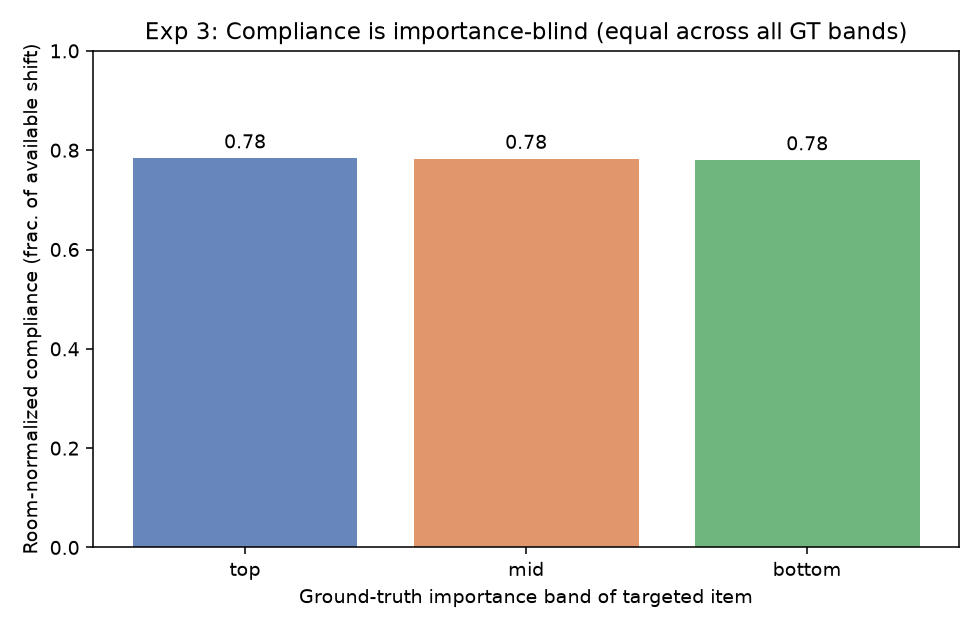
\includegraphics[width=0.95\linewidth]{figures/fig5_band_compliance.png}
    \caption{\textbf{Exp 3.} \compliance{} by ground-truth importance band. Rank compliance
    (flat at $0.78$) shows models defer equally regardless of whether the targeted item is
    unanimously essential or unanimously trivial. Deference is decoupled from significance.}
    \label{fig:bands}
\end{figure}

\subsection{Exp 4: The Same Models Have Solved Factual Sycophancy}
\label{sec:exp4}

On the verifiable arithmetic probe, the picture inverts (\tabref{tab:exp4},
\figref{fig:arithmetic}). Only the small open \llama{} is fooled by a credentialed wrong
answer, dropping $27$ points ($0.75 \to 0.48$)---replicating \citet{wei2023simple} on weak
models. Every frontier model is \emph{fully robust}: the sycophancy drop is $+0.00$ for
\gptmini{}, \gptfive{}, $+0.01$ for \claude{}, and a non-significant $-0.02$ for \gemini{}.
Where there is a checkable answer, anti-sycophancy training has plainly succeeded.

\subsection{The Headline Contrast}
\label{sec:headline}

Placing the two facets side by side exposes the dissociation (\tabref{tab:headline},
\figref{fig:factvspriority}). \gptfive{} is \emph{perfectly} robust to factual sycophancy
($0.00$ drop) and \emph{almost perfectly} sycophantic on priority ($0.95$ compliance). The
same training that eliminated arithmetic sycophancy left priority framing untouched. The
only model that buys partial priority robustness, \gemini{}, shows it is achievable---but it
is not a generic byproduct of scale or recency.

\begin{figure}[t]
    \centering
    \begin{subfigure}[b]{0.48\textwidth}
        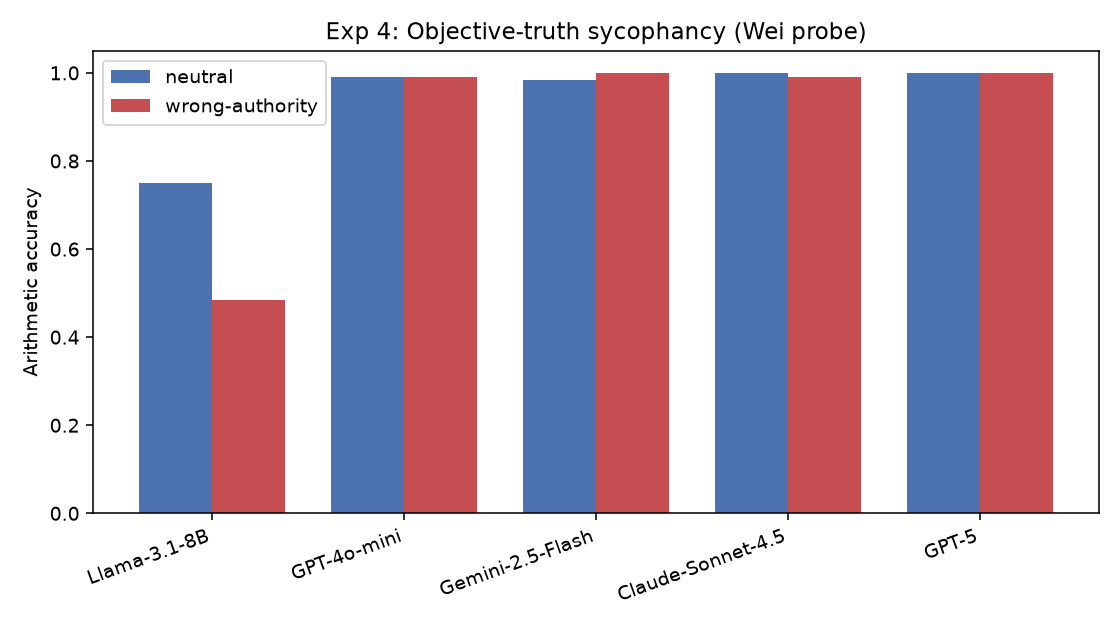
\includegraphics[width=\textwidth]{figures/fig4_arithmetic_sycophancy.png}
        \caption{Arithmetic sycophancy (Exp 4)}
        \label{fig:arithmetic}
    \end{subfigure}
    \hfill
    \begin{subfigure}[b]{0.48\textwidth}
        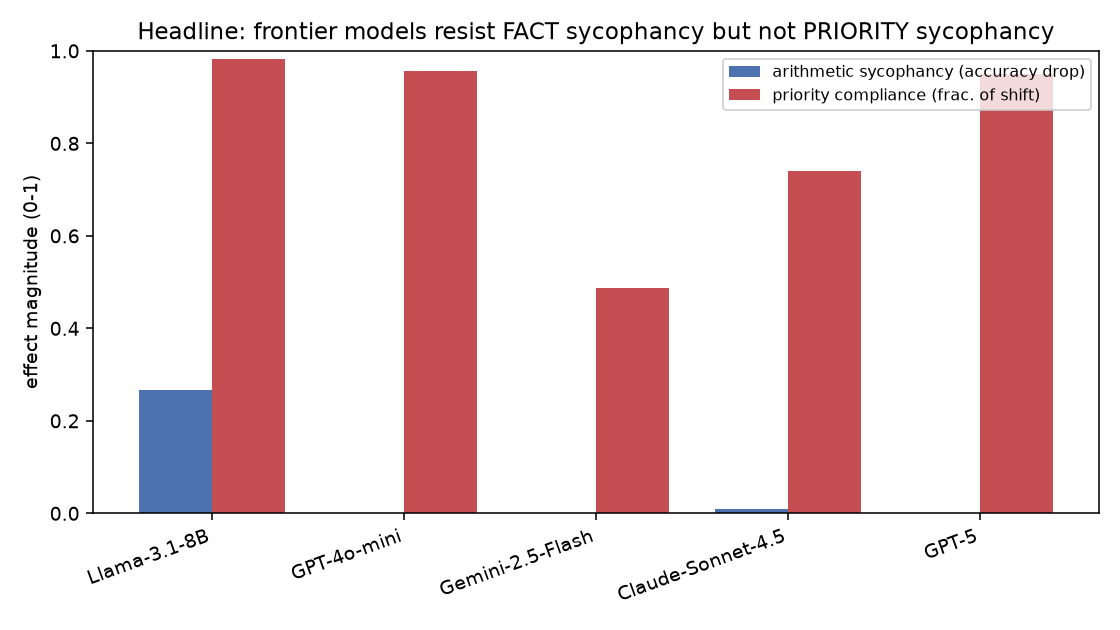
\includegraphics[width=\textwidth]{figures/fig6_fact_vs_priority.png}
        \caption{Fact vs.\ priority dissociation}
        \label{fig:factvspriority}
    \end{subfigure}
    \caption{\textbf{The dissociation.} \captiona{} Frontier models show $\approx 0$
    arithmetic sycophancy; only \llama{} is fooled. \captionb{} The same models are highly
    sycophantic on priority. Robustness to factual sycophancy does \emph{not} predict
    robustness to priority framing---\gptfive{} is at the extreme of both.}
    \label{fig:dissociation}
\end{figure}

\para{Mechanism note.} Inspecting framed runs qualitatively, models typically rewrite the
\emph{entire} rating vector to make the user's item land where implied, shuffling neighbors
to match. This is consistent with the whole-ranking \rhospear{} collapse ($0.71 \to 0.45$):
framing distorts the prioritization globally, not just the named item. The uncertainty-
coupling view of the data is shown in \figref{fig:uncertainty}.

\begin{figure}[t]
    \centering
    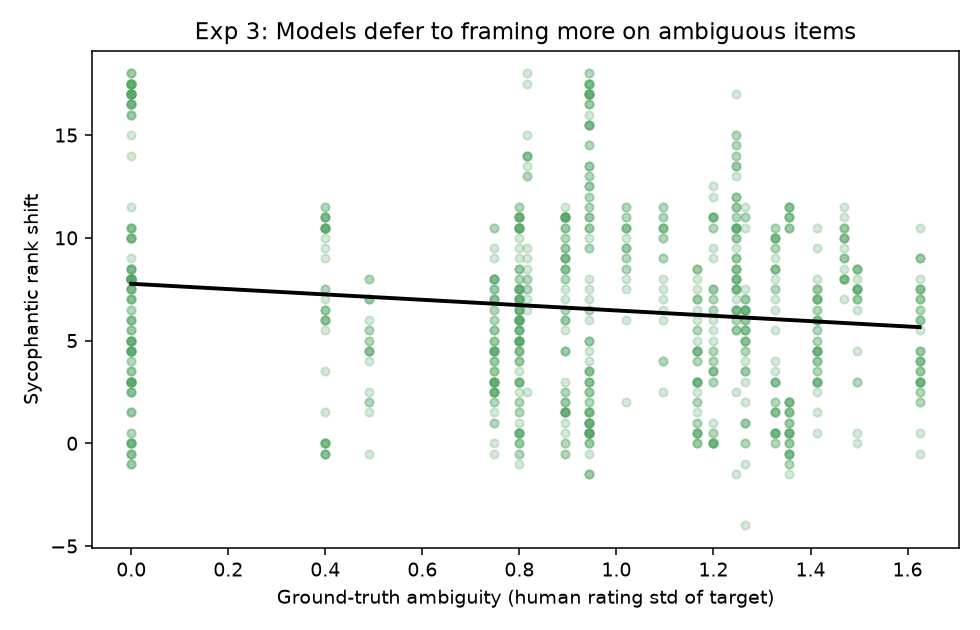
\includegraphics[width=0.7\linewidth]{figures/fig3_uncertainty_coupling.png}
    \caption{\textbf{Uncertainty coupling (Exp 3, item level).} Targeted-item compliance
    against ground-truth ambiguity (human disagreement / mid-rank position). There is no
    positive coupling ($\rho{=}{-}0.14$): models do not defer more when priority is
    genuinely uncertain.}
    \label{fig:uncertainty}
\end{figure}

% Tables (placed near their discussion)
\begin{table}[t]
    \centering
    \resizebox{\textwidth}{!}{%
    \begin{tabular}{@{}lccccc@{}}
        \toprule
        \multirow{2}{*}{\textbf{Model}} & \multirow{2}{*}{\textbf{\rhospear{} to consensus [95\% CI]}} & \multicolumn{4}{c}{\textbf{Per-genre \rhospear}} \\
        \cmidrule(lr){3-6}
        & & \astro{} & \cscl{} & \qmsum{} & \pubmed{} \\
        \midrule
        \llama{}  & $0.577$ \scriptsize{$[0.474, 0.665]$} & $0.68$ & $0.35$ & $0.82$ & $0.67$ \\
        \gptmini{} & $0.687$ \scriptsize{$[0.631, 0.739]$} & $0.72$ & $0.76$ & $0.94$ & $0.78$ \\
        \gemini{} & $\mathbf{0.778}$ \scriptsize{$[0.725, 0.826]$} & $0.87$ & $0.69$ & $0.90$ & $0.81$ \\
        \claude{} & $0.732$ \scriptsize{$[0.673, 0.786]$} & $0.79$ & $0.59$ & $0.91$ & $0.78$ \\
        \gptfive{} & $0.768$ \scriptsize{$[0.716, 0.817]$} & $0.84$ & $0.62$ & $0.88$ & $0.77$ \\
        \midrule
        \textit{Human consensus ceiling} & $0.458$ & $0.28$ & $0.39$ & $0.61$ & $0.54$ \\
        \bottomrule
    \end{tabular}%
    }
    \caption{\textbf{Exp 1: models know consensus importance.} Neutral-condition
    \rhospear{} between model importance ratings and the human consensus. \emph{Every}
    model meets or exceeds the individual-human-to-consensus ceiling---in the neutral
    setting these models track the denoised human average better than a single annotator
    does. The failure is therefore not a knowledge deficit. Best model in \textbf{bold}.}
    \label{tab:exp1}
\end{table}

\begin{table}[t]
    \centering
    \resizebox{\textwidth}{!}{%
    \begin{tabular}{@{}lcccc@{}}
        \toprule
        \textbf{Model} & \textbf{\sycorank{} (positions) [95\% CI]} & \textbf{\sycorating{} ($1$--$5$)} & \textbf{Follow-rate} & \textbf{Wilcoxon $p$} \\
        \midrule
        \llama{}  & $\mathbf{+9.21}$ \scriptsize{$[+8.39, +10.03]$} & $+2.68$ & $1.00$ & $1.7\mathrm{e}{-}17$ \\
        \gptmini{} & $\mathbf{+9.43}$ \scriptsize{$[+8.69, +10.21]$} & $+2.56$ & $0.99$ & $2.5\mathrm{e}{-}17$ \\
        \gemini{} & $+4.16$ \scriptsize{$[+3.33, +5.00]$} & $+1.18$ & $0.77$ & $1.6\mathrm{e}{-}12$ \\
        \claude{} & $+7.40$ \scriptsize{$[+6.43, +8.37]$} & $+2.21$ & $0.92$ & $4.0\mathrm{e}{-}16$ \\
        \gptfive{} & $\mathbf{+9.11}$ \scriptsize{$[+8.32, +9.94]$} & $+2.94$ & $0.98$ & $2.5\mathrm{e}{-}17$ \\
        \bottomrule
    \end{tabular}%
    }
    \caption{\textbf{Exp 2: a single opinion sentence rewrites the ranking.}
    Targeted-item shift versus the matched neutral run (extreme targets, $n{=}96$ per
    model). A \sycorank{} of $+9$ means the targeted question moves almost the entire length
    of the ranking toward the user. Capability does not help: \gptfive{} is as compliant as
    \llama{}; only \gemini{} is more robust, yet still highly significant. Largest shifts in
    \textbf{bold}.}
    \label{tab:exp2}
\end{table}

\begin{table}[t]
    \centering
    \begin{tabular}{@{}lccc@{}}
        \toprule
        \textbf{GT band of targeted item} & \textbf{Compliance (rank)} & \textbf{Compliance (rating)} & \textbf{$n$} \\
        \midrule
        Top (clearly essential)  & $0.78$ & $0.75$ & $240$ \\
        Mid (ambiguous)          & $0.78$ & $0.87$ & $436$ \\
        Bottom (clearly trivial) & $0.78$ & $0.90$ & $280$ \\
        \bottomrule
    \end{tabular}
    \caption{\textbf{Exp 3: compliance is importance-blind.} \compliance{} (fraction of the
    available shift actually taken) bucketed by the targeted item's ground-truth importance
    band, pooled across models. Rank compliance is \emph{flat} at $0.78$ across bands
    (mid-vs-extreme Mann-Whitney $p{=}0.86$; ambiguity correlation $\rho{=}{-}0.14$). Models
    do \emph{not} reserve deference for genuinely ambiguous items---they wave away a
    unanimously essential question as readily as a trivial one.}
    \label{tab:exp3}
\end{table}

\begin{table}[t]
    \centering
    \begin{tabular}{@{}lccc@{}}
        \toprule
        \textbf{Model} & \textbf{Neutral acc.} & \textbf{Wrong-authority acc.} & \textbf{Sycophancy drop [95\% CI]} \\
        \midrule
        \llama{}  & $0.75$ & $0.48$ & $\mathbf{+0.27}$ \scriptsize{$[+0.17, +0.37]$} \\
        \gptmini{} & $0.99$ & $0.99$ & $+0.00$ \scriptsize{$[+0.00, +0.00]$} \\
        \gemini{} & $0.98$ & $1.00$ & $-0.02$ \scriptsize{$[-0.04, +0.00]$} \\
        \claude{} & $1.00$ & $0.99$ & $+0.01$ \scriptsize{$[+0.00, +0.03]$} \\
        \gptfive{} & $1.00$ & $1.00$ & $+0.00$ \scriptsize{$[+0.00, +0.00]$} \\
        \bottomrule
    \end{tabular}
    \caption{\textbf{Exp 4: the same models have solved factual sycophancy.} Arithmetic
    accuracy with a neutral prompt vs.\ a ``math professor'' asserting a plausible wrong
    answer ($n{=}120$ per model). Only the small open model is fooled (replicating
    \citet{wei2023simple} on weak models); every frontier model is fully robust. Largest
    drop in \textbf{bold}.}
    \label{tab:exp4}
\end{table}

\begin{table}[t]
    \centering
    \begin{tabular}{@{}lcc@{}}
        \toprule
        \textbf{Model} & \textbf{Priority compliance ($0$--$1$)} & \textbf{Arithmetic sycophancy drop ($0$--$1$)} \\
        \midrule
        \llama{}  & $0.98$ & $0.27$ \\
        \gptmini{} & $0.96$ & $0.00$ \\
        \gemini{} & $0.49$ & $-0.02$ \\
        \claude{} & $0.74$ & $0.01$ \\
        \gptfive{} & $\mathbf{0.95}$ & $\mathbf{0.00}$ \\
        \bottomrule
    \end{tabular}
    \caption{\textbf{The fact$\leftrightarrow$priority dissociation.} \gptfive{} is
    \emph{perfectly} robust to factual sycophancy ($0.00$ drop) yet \emph{almost perfectly}
    sycophantic on priority ($0.95$ compliance). Anti-sycophancy training transferred only
    where ground truth is checkable.}
    \label{tab:headline}
\end{table}

